\chapter{Arquitetura da Aplicação}

A arquitetura da aplicação a desenvolver é definida por quatro módulos principais: Catálogo de clientes, Catálogo de produtos, Faturação Global e Vendas por Filial, cujas fontes de dados são três ficheiros de texto detalhados abaixo.
 
\paragraph{}
No ficheiro \textbf{Produtos.txt} cada linha representa o código de um produto vendável no hipermercado, sendo cada código formado por duas letras maiúsculas e 4 dígitos (que representam um inteiro entre 1000 e 1999), como no exemplo: 

\begin{verbatim}
AB9012
XY1185
BC9190
\end{verbatim}

O ficheiro de produtos contém cerca de 200.000 códigos de produto. 

\paragraph{}
No ficheiro \textbf{Clientes.txt} cada linha representa o código de um cliente identificado no hipermercado, sendo cada código de cliente formado por uma letra maiúscula e 4 dígitos que representam um inteiro entre 1000 e 5000, segue um exemplo: 

\begin{Verbatim}
F2916
W1219
F2915
\end{Verbatim}

O ficheiro de clientes contém cerca de 20.000 códigos de cliente. 

\paragraph{}
O ficheiro \textbf{Vendas\_1M.txt}, no qual cada linha representa o registo de uma venda efectuada numa qualquer das 3 filiais da Cadeia de Distribuição. Cada linha (a que chamaremos compra ou venda, o que apenas depende do ponto de vista) será formada por um código de produto, um preço unitário decimal (entre 0.0 e 999.99), o número inteiro de unidades compradas (entre 1 e 200), a letra \textbf{N} ou \textbf{P} conforme tenha sido uma compra \textbf{Normal} ou uma compra em \textbf{Promoção}, o código do cliente, o mês da compra (1 ... 12) e a filial (de 1 a 3) onde a venda foi realizada, como se pode verificar nos exemplos seguintes:
 
 \begin{Verbatim}
KR1583 77.72 128 P L4891 2 1
QQ1041 536.53 194 P X4054 12 3
OP1244 481.43 67 P Q3869 9 1
JP1982 343.2 168 N T1805 10 2
IZ1636 923.72 193 P T2220 4 2 
 \end{Verbatim}
 
O ficheiro de vendas inicial, \textbf{Vendas\_1M.txt} , conterá 1.000.000 (1 milhão) de registos de vendas realizadas nas 3 filiais da cadeia de distribuição. Existirão também os ficheiros  \textbf{Vendas\_3M.txt} e  \textbf{Vendas\_5M.txt} utilizados para as questões de performance da aplicação. 

\newpage 
\paragraph{}
A aplicação possuiu uma arquitectura tal como apresentado na figura seguinte, em que se identificam as fontes de dados, a sua leitura e os módulos de dados a construir: 

\begin{figure}[h!]
	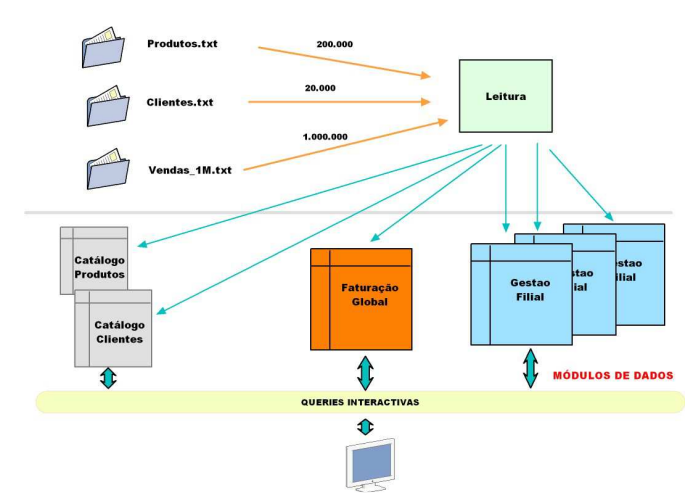
\includegraphics[scale=0.8]{arquiteturaproj.png}  
	\caption{Arquitetura da aplicação}  
\end{figure}


\chapter{Diagrama de classes}
De seguida é apresentado o Diagrama de classes gerado no BlueJ com os ficheiros .java usados. 

\begin{figure}[h!]
	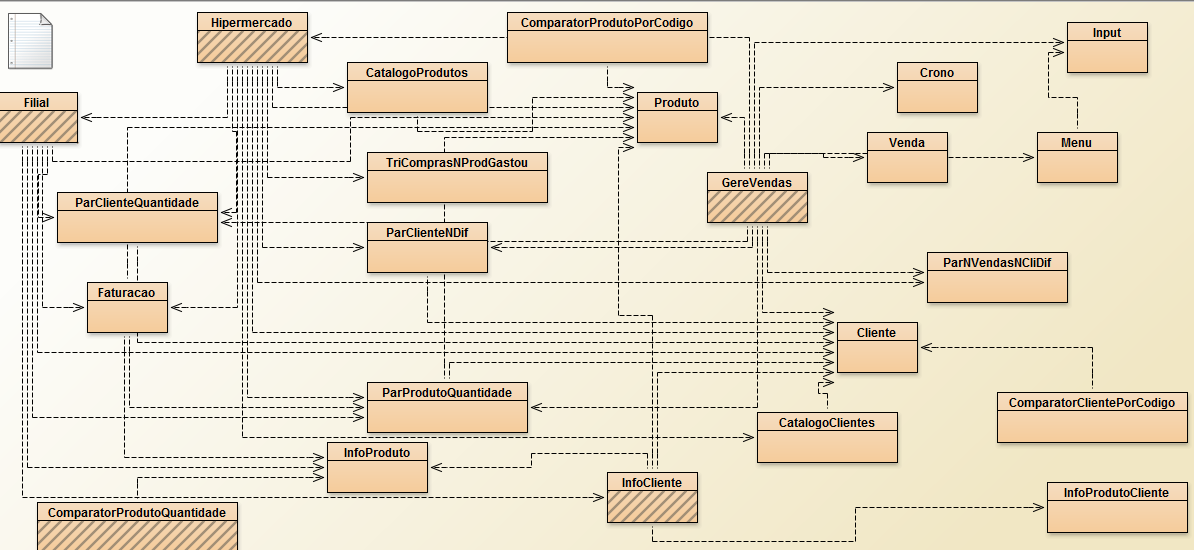
\includegraphics[scale=0.55]{diagramaclasses.png}  
	\caption{Diagrama de classe do Blue J }  
\end{figure}

\chapter{Módulos de dados}

\section{Catálogo de Clientes}
É o módulo de dados onde são guardados os códigos de todos os clientes do ficheiro \textbf{Clientes.txt}, organizados por índice alfabético;

\subsection{Classe CatalogoClientes} 

Para guardar os clientes presentes no ficheiro de clientes.txt, criámos a classe \color{blue} \textbf{CatalogoClientes} \color{black} que
irá guardar a lista de todos os clientes presentes no ficheiro. Utilizando \color{blue} HashSet \color{black} que guarda todos os códigos de cliente do tipo \color{blue} \textbf{String} \color{black} e retira os repetidos, proporcionando assim uma pesquisa rápida.

A classe \color{blue} \textbf{CatalogoClientes} \color{black} servirá também para validar os clientes.

\begin{Verbatim}
private Set<Cliente> catalogoClientes;
\end{Verbatim}


\subsection{Classe Cliente}
A classe \color{blue} \textbf{Cliente} \color{black} foi implementada para guardar o código de cada cliente. Foi utilizada a classe especial em Java que é responsável por fazer comparações de objetos, que é a classe \color{blue} Comparable \color{black}. Usada como padrão de comparação, serve para comparar o tipo de objectos para os quais o objeto  Cliente pode ser comparado. 

 

\begin{Verbatim}
public class Cliente implements Comparable<Cliente> {

	private String codigo_cliente;
\end{Verbatim}



\subsection{Classe InfoCliente}

Esta classe foi criada para guardar informações relativas ao cliente, tais como o dinheiro que um cliente gastou num mês, a quantidade de produtos comprados num mês, as compras efetuadas, a quantidade de compras efetuadas, total de dinheiro gasto, assim como a lista de todos os produtos comprados em modo de Promoção(P), ou em modo Normal (N).  


Fica aqui o código que define as variáveis de instância da classe InfoCliente:

\begin{Verbatim}
class InfoCliente {
private double[] dinheiroGastoMes;
private int[] totalCompradoMes;
private int [] vendas;
private int totalComprado;
private double totalGasto;
private Map <Produto,InfoProdutoCliente> produtosComprados[]; // modos N P

\end{Verbatim}


Esta classe contém os construtores, clone e os respetivos set e get definidos que servirão de auxilio noutras classes. 



\section{Catálogo de Produtos}

 Módulo de dados onde são guardados os códigos de todos os produtos do ficheiro \textbf{Produtos.txt}, organizados por índice alfabético, o que irá permitir, de forma eficaz, saber quais são os produtos cujos códigos começam por uma dada letra do alfabeto e saber quantos produtos são contabilizados. 
 
 \subsection{Classe CatalogoProdutos}
 
 Para guardar os produtos presentes no ficheiro de produtos.txt, criámos a classe \color{blue} \textbf{CatalogoProdutos} \color{black} que
 irá guardar a lista de todos os produtos presentes no ficheiro. Utilizando \color{blue} HashSet \color{black} que guarda todos os códigos de produto do tipo \color{blue} \textbf{String} \color{black} e retira os repetidos, proporcionando assim uma pesquisa rápida.
 
 A classe \color{blue} \textbf{CatalogoProdutos} \color{black} servirá também para validar os produtos.

\begin{verbatim}
private Set<Produto> catalogoProdutos;
\end{verbatim}

\subsection{Classe Produto}

A classe \color{blue} \textbf{Produto} \color{black} foi implementada para guardar o código de cada produto. Esta classe é semelhante à classe Cliente. 


\begin{verbatim}
public class Produto implements Comparable<Produto> {

private String codigo_produto;
\end{verbatim}


\subsection{Classe InfoProduto}
A classe InfoProduto serve para guardar as informações relativas ao produto, tais como a quantidade de um produto em determinado mes numa filial, a quantidade total, o total faturado, o faturado num mes em determinada filial, e o total de vendas efetuadas.  

\begin{verbatim}
public class InfoProduto {
private int [][] quantidade; // [12][3] mes, filial
private int quantidadeTotal;
private double [][] faturado; // [12][3] mes, filial
private double totalFaturado;
private int[][] vendas;
\end{verbatim}







\section{Faturação Global}

Módulo de dados que contém as estruturas de dados responsáveis pela resposta a questões quantitativas que relacionam os produtos às suas vendas mensais, em modo Normal (N) ou em Promoção (P), para cada um dos casos guardando o número de vendas e o valor total de faturação de cada um destes tipos. Este módulo refecencia todos os produtos, mesmo os que nunca foram vendidos, não contém qualquer referência a clientes, mas é capaz de distinguir os valores obtidos em cada filial. 

\subsection{Classe Faturacao}

A classe  \color{blue} \textbf{Faturacao} \color{black} serve para guardar o número de vendas, total faturado, e os produtos vendidos, assim como os não vendidos 

\begin{verbatim}
public class Faturacao {
private int totalVendas;
private double totalFaturado;
private HashMap<Produto, InfoProduto> produtosVendidos;
\end{verbatim}



\section{Gestão da Filial}

Módulo de dados que, a partir dos ficheiros lidos, contém as estruturas de dados adequadas à representação dos relacionamentos, fundamentais para a aplicação, entre produtos e clientes, ou seja, para cada produto, saber quais os clientes que o compraram, quantas unidades cada um comprou, o mês e a filial.

 Para a estruturação optimizada dos dados deste módulo de dados tivemos em atenção que pretendemos ter o histórico de vendas organizado por filial para uma melhor análise, nunca esquecendo que existem 3 filiais nesta cadeia. 

\subsection{Classe Filial}
Guarda a informação de todos os cliente quer tenham comprado ou não. 

\begin{verbatim}
public class Filial {
private Map<Cliente,InfoCliente> informacaoClientes; 
\end{verbatim}

\section{Classe Hipermercado }

Esta é a classe principal onde se guardam todas as informações relativas ao funcionamento do hipermercado. 

\begin{verbatim}

public class Hipermercado implements Serializable {

private CatalogoClientes clientes;
private CatalogoProdutos produtos;
private Filial filiais[];
private Faturacao faturacao;
private int vendaserradas;
private int comprasnulas;
private double faturacaoglobal;
\end{verbatim}

\section{GereVendas}

Todo o programa é inicializado nesta função, o hipermercado é inicializado nesta classe que posteriormente iniciará as restantes classes, o menu principal do programa começa  a executar permitindo assim ao utilizador navegar pelo programa e executar as queries e obter os resultados que quiser consultar.
Esta classe contém quais os ficheiros para leitura, assim como o caminho para eles assim como o último estado guradado. 

\section{Venda}

A classe Venda simplifica os dados introduzidos, sendo que assim os dados deixam de ser apenas uma string e passam a ser uma venda concreta para o programa poder consultar livremente e fazer as devidas inserções nas estruturas de forma mais simples.
Esta classe é tambem responsável pela validação de todas as vendas introduzidas.


\begin{verbatim}
public class Venda implements Serializable{

private String codigoProduto;
private String codigoCliente;
private char modoDeCompra;
private int mes;
private int filial;
private double preco;
private int quantidade;
\end{verbatim}



\chapter{Interface com utilizador}

Nesta secção apresenta-se a interface com o utilizador, fazendo algumas considerações sobre as decisões tomadas.
Ao iniciar o programa GereVendas, o utilizador tem um menu que lhe permite carregar ou não o último estado do programa, isto é o ficheiro hipermercado.dat. 

\begin{figure}[h!]
	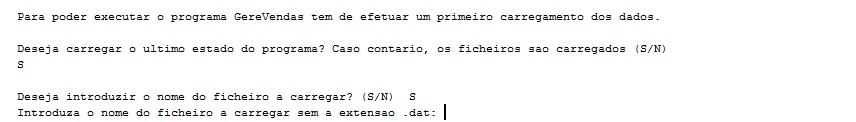
\includegraphics[scale=1]{IntroduzirUmFicheiroStream.jpg}  
	\caption{Inicio da execução do programa }  
\end{figure}

Se não quiser carregar o último estado do programa carrega os ficheiros Clientes.txt Produtos.txt automáticamente e pede para escolher qual o ficheiro de Vendas que pretende escolher, se escolher a opção N (não) carrega o ficheiro de Vendas\_1M: 

\begin{figure}[h!]
	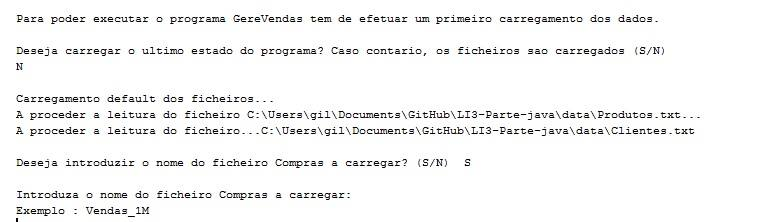
\includegraphics[scale=0.65]{menunao.jpg}  
	\caption{Escolha da opção N (não) }  
\end{figure}

Depois do carregamento dos ficheiros de dados é apresentado o seguinte menu com as 5 opções: 


\begin{itemize}
	\item Carregar Programa - esta opção permite carregar o ficheiro hipermercado.dat
	\item Gravar estado do programa - esta opção permite gravar o os ficheiros no hipermercado.dat 
	\item Consultas Estatisticas - Apresenta ao utilizador os dados referentes ao último ficheiro de vendas lido,
	designadamente, nome do ficheiro, número total de registos de venda errados,
	número total de produtos, total de diferentes produtos comprados, total de não
	comprados, número total de clientes e total dos que realizaram compras, total de
	clientes que nada compraram, total de compras de valor total igual a 0.0 e
	facturação total. Apresenta também os números gerais respeitantes aos dados
	atuais já registados nas estruturas, designadamente, número total de compras por mês (não é a facturação); Facturação total por mês (valor total das compras/vendas) para cada filial e o valor total global; Número de distintos clientes que compraram em cada mês (não interessa quantas vezes o cliente comprou mas apenas quem de facto comprou); 

	\item Consultas Interativas  - Abrirá um menu com as queries numeradas de 1 a 9, basta escolher o numero da querie que o utilizador pretende executar e seguir os passos. 
\end{itemize}

	
\begin{figure}[h!]
	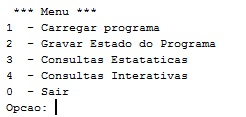
\includegraphics[scale=1.5]{MenuInicial.jpg}  
	\caption{Menu Inicial }  
\end{figure}

Quando se escolhe a opção 3 aparece o seguinte menu: 
\begin{figure}[h!]
	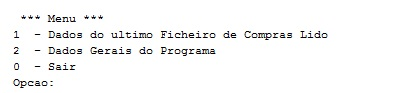
\includegraphics[scale=1]{ConsultasEstatisticas.jpg}  
	\caption{Opção 3 - Consulta das Estatisticas }  
\end{figure}

Quandos se escolhe o menu das queries (4) 
\begin{figure}[h!]
	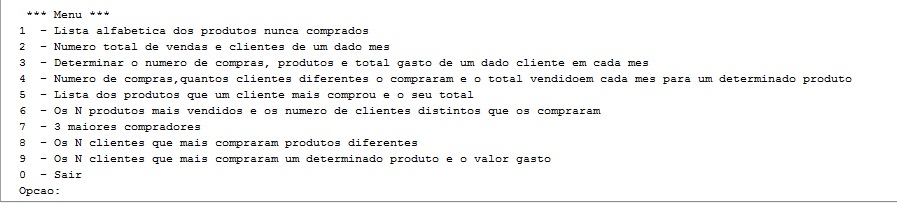
\includegraphics[scale=0.9]{ConsultasIterativas}  
	\caption{Opção 4 - Consulta das queries }  
\end{figure}

A partir daqui a escolha de um número de 0 a 9 vai implicar a execução de determinada querie, conforme o pretendido pelo utilizador. 

\chapter{Resultados e comentários sobre os testes de performance}

Depois de desenvolver e codificar todo o projeto foi-nos proposto realizar alguns testes de performance que consistem em comparar os tempos de carregamneto de ficheiros e de execução das queries 5, 6, 7, 8 e 9.

O programa foi corrido num computador ASUS k55v com um processador intel(R) core(TM) i5-3210M CPU@2.50GHz, memória RAM 6 GB onde 5.89 são utilizáveis, sistema operativos de 64 bits, processador baseado em x64.A máquima possui uma placa gráfica GEFORCE* GT 630M* 2GB e um disco rigido de HDD 500GB, o windows utilizado pela máquina é o windows 10. 

 
\section{Performance Leitura dos Ficheiros}

\par Para verificar qual a melhor classe a usar para fazer a leitura dos ficheiros corremos testes para as classes
\color{blue} \textbf{BufferedReader} \color{black} e para a classe \color{blue} \textbf{Scanner} \color{black} realizando testes
fazendo parsing da string e criando instância da class \color{blue} \textbf{Venda} \color{black} e testes sem parsing.
\par De seguida ficam tabelas com os resultados obtidos e também dois gráfico para comparação de resultados.

Para cada uma das situações corremos 5 vezes, para os ficheiros Vendas\_1M, Vendas\_3M, Vendas\_5M , no final calculamos a média destas 5 execuções e foi o tempo que se registou.

\begin{figure}[h!]
	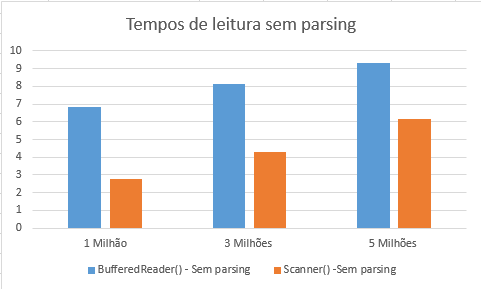
\includegraphics[scale=1]{graficosemparsing}  
	\caption{Gráfico de tempos de leitura sem parsing }  
\end{figure}

\begin{figure}[h!]
	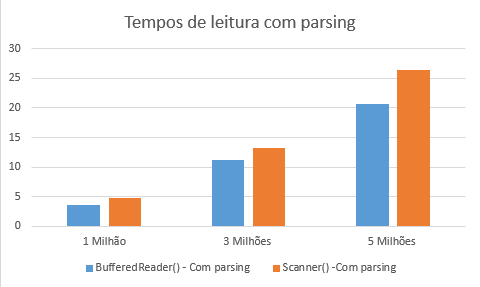
\includegraphics[scale=1]{graficocomparsing}  
	\caption{Gráfico com os tempos de leitura com parsing }  
\end{figure}

\par Assim pode-se concluir que apesar de \color{blue} \textbf{Scanner} \color{black} ser mais rápido do que  \color{blue} \textbf{BufferedReader} \color{black} na execução do programa sem parsing, o mais vantajoso para este caso é a utilização do \color{blue} \textbf{BufferedReader} \color{black}. Pois como se pode verificar no gráfico de tempos de leitura com parsing o  \color{blue} \textbf{BufferedReader} \color{black} apresenta menlhores resultados do que na classe \color{blue} \textbf{Scanner} \color{black}. 


\section{Performance Queries }
Para testar a performance das queries foi proposto que fossem substituidas as estruturas inciais por outras. 


No inicio a estrutura utilizada no catalogo de clientes e de produtos foi um HashSet e mudou-se para um TreeSet. 


Nas classes Faturação, Filial e InfoCliente inicialmente utilizou-se uma HashMap depois mudou-se para uma TreeMap. 

Para medir os tempos executamos as queries 6,7,8 e 9 num total de 5 medições fazendo de seguida a média.


Na query 8 utilizamos o códiGo de cliente Z5000 . 

Na querie 9 utilizamos o códiGo AF1184. 

\par De seguida apresentamos a tabela dos tempos registados seguido de um gráfico que irá ajudar na conclusão destes testes de performance das diferentes estruturas.

\begin{figure}[h!]
	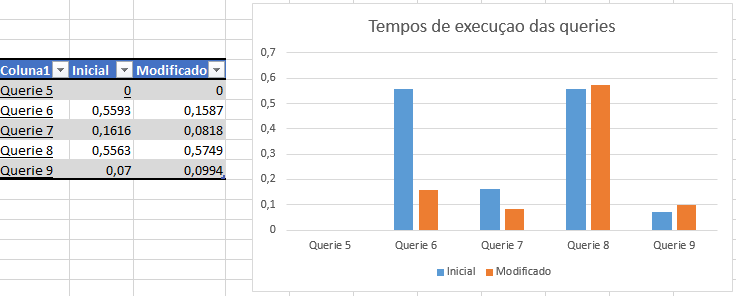
\includegraphics[scale=0.8]{graficoqueries}  
	\caption{Tabela e gráfico com a execução dos tempos das diferentes estruturas utilizadas }  
\end{figure}
  	